\documentclass[border=2pt]{standalone}
\usepackage[T1]{fontenc}
\usepackage{newtxtext,newtxmath}
\usepackage{tikz}
\usetikzlibrary{arrows.meta}
\definecolor{hesp}{HTML}{4C72B0}
\definecolor{llm}{HTML}{DD8452}
\definecolor{env}{HTML}{8C8C8C}
\definecolor{ver}{HTML}{55A868}
\begin{document}
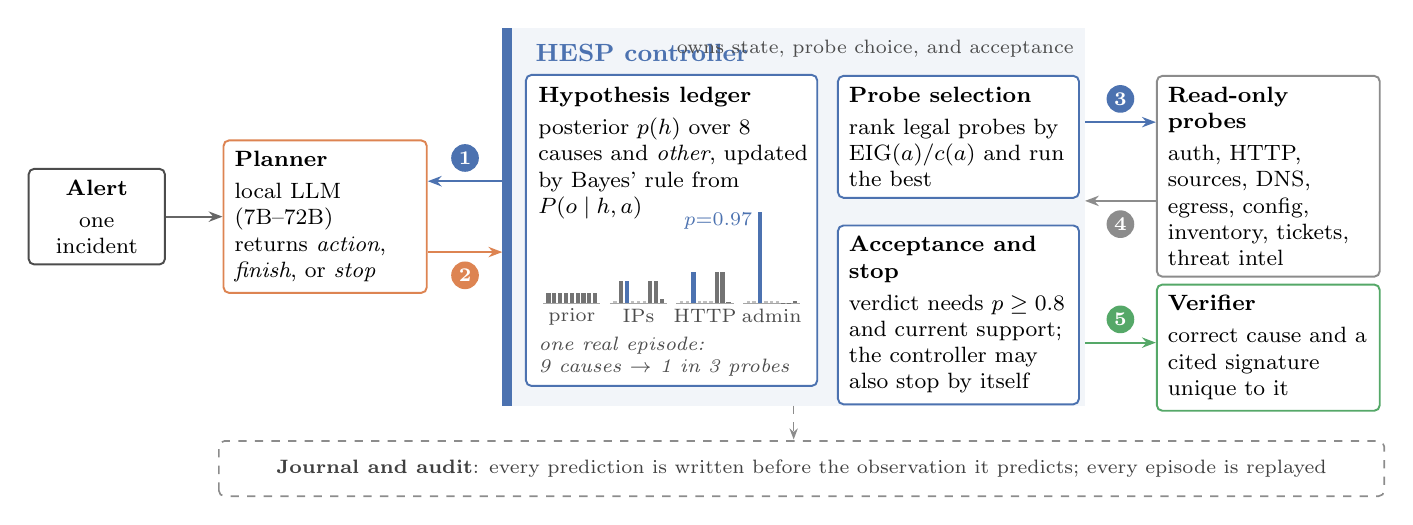
\begin{tikzpicture}[font=\footnotesize,
  box/.style={draw=#1, line width=0.7pt, fill=white, rounded corners=2pt, align=flush left, inner sep=4pt},
  lab/.style={font=\scriptsize, text=black!70, inner sep=1pt},
  flow/.style={-{Stealth[length=5pt]}, line width=0.8pt, draw=#1},
  step/.style={circle, fill=#1, text=white, font=\scriptsize\bfseries, inner sep=0pt, minimum size=10pt},
  axis/.style={draw=black!35, line width=0.4pt},
  bar/.style={fill=black!55}, win/.style={fill=hesp}, elim/.style={fill=black!25}]

% ---- controller region (x 6.0..13.4)
\fill[hesp!7] (6.0,0.75) rectangle (13.4,5.55);
\fill[hesp] (6.0,0.75) rectangle (6.12,5.55);
\node[font=\small\bfseries, text=hesp, anchor=north west] at (6.3,5.47) {HESP controller};
\node[lab, anchor=north east] at (13.3,5.44) {owns state, probe choice, and acceptance};

% ledger (x 6.3..10.0) with one real episode
\draw[hesp, line width=0.7pt, fill=white, rounded corners=2pt] (6.3,1.0) rectangle (10.0,4.95);
\node[anchor=north west, align=flush left, text width=3.45cm, inner sep=0pt] at (6.45,4.8)
  {\textbf{Hypothesis ledger}\\[2pt] posterior $p(h)$ over 8 causes and \textit{other}, updated by Bayes' rule from $P(o\mid h,a)$};
\draw[axis] (6.520,2.050) -- (7.246,2.050);
\fill[bar] (6.560,2.050) rectangle (6.614,2.183);
\fill[bar] (6.634,2.050) rectangle (6.688,2.183);
\fill[bar] (6.708,2.050) rectangle (6.762,2.183);
\fill[bar] (6.782,2.050) rectangle (6.836,2.183);
\fill[bar] (6.856,2.050) rectangle (6.910,2.183);
\fill[bar] (6.930,2.050) rectangle (6.984,2.183);
\fill[bar] (7.004,2.050) rectangle (7.058,2.183);
\fill[bar] (7.078,2.050) rectangle (7.132,2.183);
\fill[bar] (7.152,2.050) rectangle (7.206,2.183);
\node[lab, anchor=north] at (6.883,2.020) {prior};
\draw[axis] (7.366,2.050) -- (8.092,2.050);
\fill[elim] (7.411,2.050) rectangle (7.455,2.080);
\fill[bar] (7.480,2.050) rectangle (7.534,2.335);
\fill[win] (7.554,2.050) rectangle (7.608,2.335);
\fill[elim] (7.633,2.050) rectangle (7.677,2.080);
\fill[elim] (7.707,2.050) rectangle (7.751,2.080);
\fill[elim] (7.781,2.050) rectangle (7.825,2.080);
\fill[bar] (7.850,2.050) rectangle (7.904,2.335);
\fill[bar] (7.924,2.050) rectangle (7.978,2.335);
\fill[bar] (7.998,2.050) rectangle (8.052,2.107);
\node[lab, anchor=north] at (7.729,2.020) {IPs};
\draw[axis] (8.212,2.050) -- (8.938,2.050);
\fill[elim] (8.257,2.050) rectangle (8.301,2.080);
\fill[elim] (8.331,2.050) rectangle (8.375,2.080);
\fill[win] (8.400,2.050) rectangle (8.454,2.442);
\fill[elim] (8.479,2.050) rectangle (8.523,2.080);
\fill[elim] (8.553,2.050) rectangle (8.597,2.080);
\fill[elim] (8.627,2.050) rectangle (8.671,2.080);
\fill[bar] (8.696,2.050) rectangle (8.750,2.442);
\fill[bar] (8.770,2.050) rectangle (8.824,2.442);
\fill[bar] (8.844,2.050) rectangle (8.898,2.070);
\node[lab, anchor=north] at (8.575,2.020) {HTTP};
\draw[axis] (9.058,2.050) -- (9.784,2.050);
\fill[elim] (9.103,2.050) rectangle (9.147,2.080);
\fill[elim] (9.177,2.050) rectangle (9.221,2.080);
\fill[win] (9.246,2.050) rectangle (9.300,3.209);
\fill[elim] (9.325,2.050) rectangle (9.369,2.080);
\fill[elim] (9.399,2.050) rectangle (9.443,2.080);
\fill[elim] (9.473,2.050) rectangle (9.517,2.080);
\fill[bar] (9.542,2.050) rectangle (9.596,2.056);
\fill[bar] (9.616,2.050) rectangle (9.670,2.056);
\fill[bar] (9.690,2.050) rectangle (9.744,2.080);
\node[lab, anchor=north] at (9.421,2.020) {admin};
\node[lab, text=hesp, anchor=east] at (9.216,3.089) {$p{=}0.97$};
\node[lab, anchor=south west, align=flush left] at (6.42,1.08) {\textit{one real episode:}\\ \textit{9 causes $\to$ 1 in 3 probes}};

% selection and acceptance (x 10.25..13.15)
\node[box=hesp, anchor=north west, text width=2.78cm] at (10.25,4.95)
  {\textbf{Probe selection}\\[2pt] rank legal probes by $\mathrm{EIG}(a)/c(a)$ and run the best};
\node[box=hesp, anchor=north west, text width=2.78cm] (acc) at (10.25,3.05)
  {\textbf{Acceptance and stop}\\[2pt] verdict needs $p\ge0.8$\\ and current support;\\ the controller may\\ also stop by itself};

% ---- alert, planner, probes, verifier
\node[box=black!70, text width=1.45cm, align=center] (alert) at (0.85,3.15) {\textbf{Alert}\\[2pt] one incident};
\node[box=llm, text width=2.3cm] (plan) at (3.75,3.15)
  {\textbf{Planner}\\[2pt] local LLM (7B--72B)\\ returns \textit{action},\\ \textit{finish}, or \textit{stop}};
\node[box=env, anchor=north west, text width=2.55cm] (probe) at (14.3,4.95)
  {\textbf{Read-only probes}\\[2pt] auth, HTTP, sources, DNS, egress, config, inventory, tickets, threat intel};
\node[box=ver, anchor=north west, text width=2.55cm] (verif) at (14.3,2.3)
  {\textbf{Verifier}\\[2pt] correct cause and a cited signature unique to it};

% ---- journal across the whole pipeline
\draw[black!45, dashed, line width=0.6pt, rounded corners=2pt] (2.4,-0.4) rectangle (17.2,0.3);
\node[font=\scriptsize, text=black!75] at (9.8,-0.05)
  {\textbf{Journal and audit}: every prediction is written before the observation it predicts; every episode is replayed};
\draw[black!45, -{Stealth[length=4pt]}, line width=0.6pt, dashed] (9.7,0.75) -- (9.7,0.32);

% ---- flows with numbered steps
\draw[flow=black!60] (alert.east) -- (plan.west);
\draw[flow=hesp] (6.0,3.6) -- node[step=hesp, above=3pt] {1} (plan.east |- 0,3.6);
\draw[flow=llm] (plan.east |- 0,2.7) -- node[step=llm, below=3pt] {2} (6.0,2.7);
\draw[flow=hesp] (13.4,4.35) -- node[step=hesp, above=3pt] {3} (14.3,4.35);
\draw[flow=env] (14.3,3.35) -- node[step=env, below=3pt] {4} (13.4,3.35);
\draw[flow=ver] (13.4,1.55) -- node[step=ver, above=3pt] {5} (14.3,1.55);
\end{tikzpicture}
\end{document}
